\section{Bayesian Decision Network}
\subsection{Definition}

\begin{frame}
\frametitle{What is a BDN?}
\begin{itemize}
\item Bayesian Networks with additional decision nodes and utility nodes
	\begin{itemize}
	\item Decision nodes hold values for different actions
	\item Utility nodes are deterministic functions of their parents
	\end{itemize}
\item BDN shows which information is required in order to make
each decision
\item and the order in which these decisions are to be made
\end{itemize}
\end{frame}

\begin{frame}
\frametitle{Causal consistency}
\begin{itemize}
\item BDN is consistent when a current decision cannot affect the past
\item Descendants of a decision node must come later in the partial order
\item A vaild BDN has a directed path connecting all decisions
\end{itemize}
\end{frame}

\subsection{Example}
\begin{frame}
\begin{columns}
\column{0.6\textwidth}
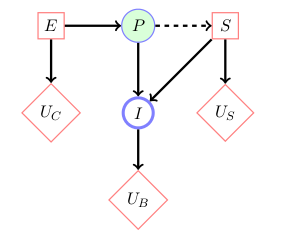
\includegraphics[width=1\textwidth]{figures/bdn}
\column{0.4\textwidth}
Partial ordering:
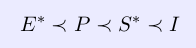
\includegraphics[width=1\textwidth]{figures/partorder}
\end{columns}
\end{frame}


\subsection{Solving a BDN}
\begin{frame}
\begin{itemize}
\item Optimal EU is given by summing over unrevealed variables and optimising over future decisions
\end{itemize}

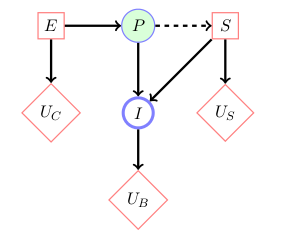
\includegraphics[width=.5\textwidth]{figures/bdn}

\begin{equation}
U(E) = \sum\limits_{P}max_s\sum\limits_{I}p(I|S,P)p(P|E)[U_S(S)+U_C(E)+U_B(I)]
\end{equation}
\end{frame}

\begin{frame}
\frametitle{Algorithm}
\begin{itemize}
	\item For each possible value of a decision node:
	\begin{itemize}
	\item Set decision node to that value
	\item Calculate the posterior probability of the parent nodes
		of the utility node, using BN inference
	\item Calculate the resulting (expected) utility for action
	\end{itemize}
	\item Return the action with the highest utility
\end{itemize}
\end{frame}

\subsection{Structure}
\begin{frame}
\frametitle{Files}
\Large\textbf{PRIMO/primo/}
\begin{itemize}
	\item core/
	\begin{itemize}
		\item BayesianDecisionNetwork.py
	\end{itemize}
	\item decision/
	\begin{itemize}
		\item DecisionNode.py
		\item UtilityNode.py
		\item UtilityTable.py
	\end{itemize}
	\item decision/make\_decision/
	\begin{itemize}
		\item Make\_Decision.py
	\end{itemize}
\end{itemize}
\end{frame}


\subsection{Literature}
\begin{frame}
\begin{itemize}
\item \textsc{Barber, David} \\ Bayesian Reasoning and Machine Learning
\end{itemize}
\end{frame}